\newpage
\section{Modellazione dei Casi d'Uso}
Dopo aver definito i requisiti funzionali e i vincoli del sistema, questa sezione illustra i casi
d'uso (use case), che descrivono in dettaglio le principali interazioni tra gli utenti e il sistema
per il raggiungimento degli obiettivi. Nella nostra analisi preliminare, abbiamo individuato quattro
attori principali che interagiscono con il sistema: Guest, Utente, Agente e Amministratore.\\
\begin{itemize}
    \item Guest: rappresenta l'utente non autenticato, che accede al sito senza effettuare il login. Questo attore ha accesso limitato, ma può comunque compiere alcune azioni di base, come
effettuare ricerche sugli Immobili e visualizzare informazioni pubbliche su di essi.
\item User: questo attore è un utente autenticato con un account registrato. Rispetto al Guest, ha funzionalità aggiuntive, come fare
offerte sugli Immobili, monitorare il proprio storico delle ricerche effettuate e ricevere notifiche in base alle preferenze che ha esibito. Queste notifiche possono esse ulteriormente personalizzata nelle impostazioni con dei filtri.
\item Agente: rappresenta l'utente che può creare e modificare gli Annunci e gli Immobili.
\item Amministratore: l'attore che gestisce l'agenzia immobiliare nella sua interezza, avendo il potere di appuntare sia Agenti che altri Amministratori. Inoltre l'amministratore può curare il catalogo di Annunci, modificando o eliminando elementi dalla lista.
\end{itemize}
Per ciascun attore, sono stati definiti i casi d'uso relativi, illustrati nei diagrammi seguenti.
Questi schemi mostrano le modalità principali d'interazione con il sistema e forniscono una
visione chiara, delineando le possibilità di interazione per ciascun tipo di utente. In questo
modo, è possibile comprendere come le funzionalità definite nei requisiti trovano applicazione
pratica all'interno delle azioni eseguibili da ciascun attore, evidenziando i passaggi chiave delle interazioni.
\newpage
\subsection*{Diagrammi Casi d'uso}

\begin{figure}[H]
\caption{Casi d'uso Guest}
\centering
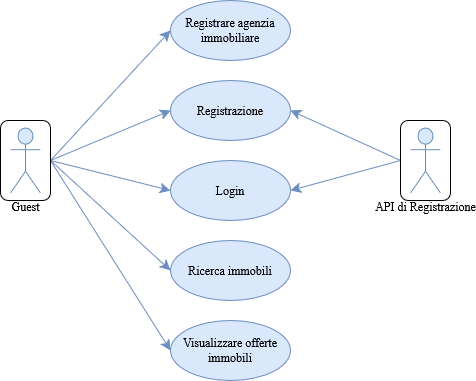
\includegraphics[width=0.8\textwidth]{Immagini/Diagrammi Casi D'uso/UseCase-Utente Non Registrato.drawio.png}
\end{figure}

\begin{figure}[H]
\centering
\caption{Casi d'uso Utente}
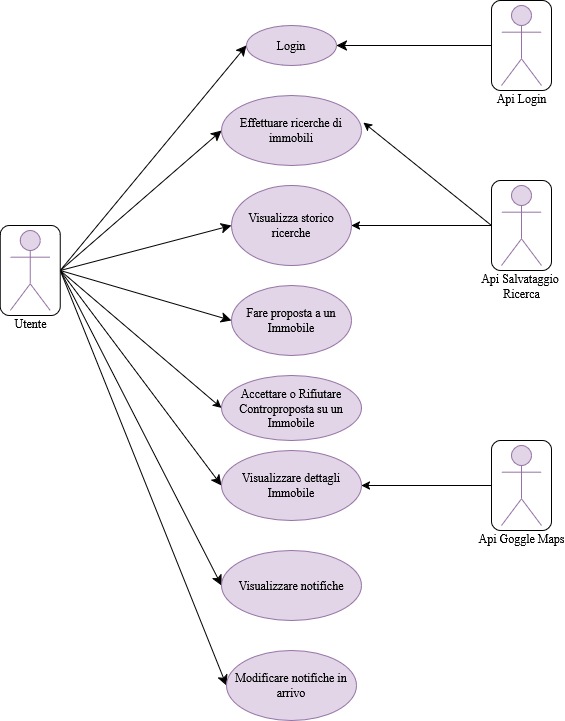
\includegraphics[width=0.8\textwidth]{Immagini/Diagrammi Casi D'uso/UseCase-Utente registrato.drawio.png}
\end{figure}

\begin{figure}[H]
\centering
\caption{Casi d'uso Agente}
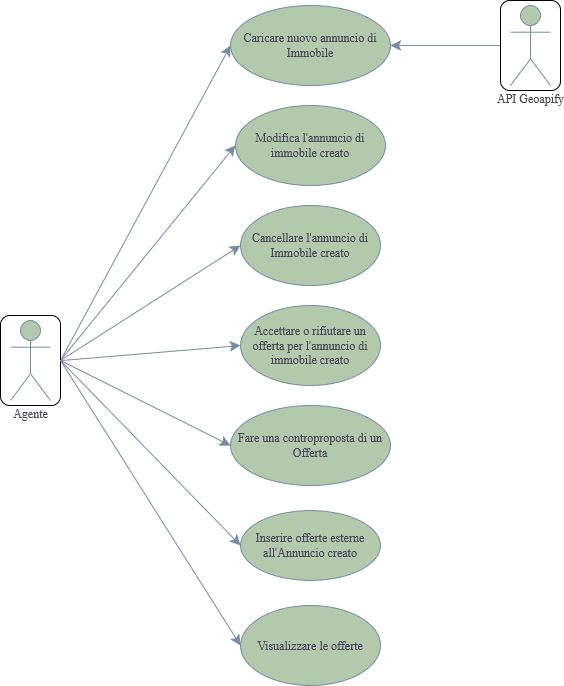
\includegraphics[width=0.8\textwidth]{Immagini/Diagrammi Casi D'uso/UseCase-Agente.drawio.png}
\end{figure}

\begin{figure}[H]
\centering
\caption{Casi d'uso Amministratore}
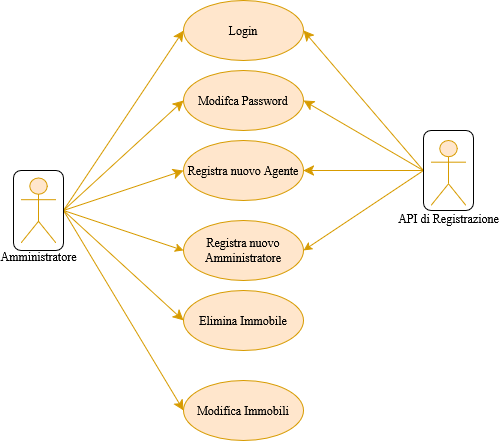
\includegraphics[width=0.8\textwidth]{Immagini/Diagrammi Casi D'uso/UseCase-Admin.drawio.png}
\end{figure}
\newpage
